% Options for packages loaded elsewhere
\PassOptionsToPackage{unicode}{hyperref}
\PassOptionsToPackage{hyphens}{url}
\PassOptionsToPackage{dvipsnames,svgnames,x11names}{xcolor}
%
\documentclass[
  ignorenonframetext,
]{beamer}
\usepackage{pgfpages}
\setbeamertemplate{caption}[numbered]
\setbeamertemplate{caption label separator}{: }
\setbeamercolor{caption name}{fg=normal text.fg}
\beamertemplatenavigationsymbolsempty
% Prevent slide breaks in the middle of a paragraph
\widowpenalties 1 10000
\raggedbottom

\usepackage{amsmath,amssymb}
\usepackage{iftex}
\ifPDFTeX
  \usepackage[T1]{fontenc}
  \usepackage[utf8]{inputenc}
  \usepackage{textcomp} % provide euro and other symbols
\else % if luatex or xetex
  \usepackage{unicode-math}
  \defaultfontfeatures{Scale=MatchLowercase}
  \defaultfontfeatures[\rmfamily]{Ligatures=TeX,Scale=1}
\fi
\usepackage{lmodern}
\usetheme[]{AnnArbor}
\usecolortheme{dolphin}
\usefonttheme{structurebold}
\ifPDFTeX\else  
    % xetex/luatex font selection
\fi
% Use upquote if available, for straight quotes in verbatim environments
\IfFileExists{upquote.sty}{\usepackage{upquote}}{}
\IfFileExists{microtype.sty}{% use microtype if available
  \usepackage[]{microtype}
  \UseMicrotypeSet[protrusion]{basicmath} % disable protrusion for tt fonts
}{}
\makeatletter
\@ifundefined{KOMAClassName}{% if non-KOMA class
  \IfFileExists{parskip.sty}{%
    \usepackage{parskip}
  }{% else
    \setlength{\parindent}{0pt}
    \setlength{\parskip}{6pt plus 2pt minus 1pt}}
}{% if KOMA class
  \KOMAoptions{parskip=half}}
\makeatother
\usepackage{xcolor}
\newif\ifbibliography
\setlength{\emergencystretch}{3em} % prevent overfull lines
\setcounter{secnumdepth}{-\maxdimen} % remove section numbering


\providecommand{\tightlist}{%
  \setlength{\itemsep}{0pt}\setlength{\parskip}{0pt}}\usepackage{longtable,booktabs,array}
\usepackage{calc} % for calculating minipage widths
\usepackage{caption}
% Make caption package work with longtable
\makeatletter
\def\fnum@table{\tablename~\thetable}
\makeatother
\usepackage{graphicx}
\makeatletter
\def\maxwidth{\ifdim\Gin@nat@width>\linewidth\linewidth\else\Gin@nat@width\fi}
\def\maxheight{\ifdim\Gin@nat@height>\textheight\textheight\else\Gin@nat@height\fi}
\makeatother
% Scale images if necessary, so that they will not overflow the page
% margins by default, and it is still possible to overwrite the defaults
% using explicit options in \includegraphics[width, height, ...]{}
\setkeys{Gin}{width=\maxwidth,height=\maxheight,keepaspectratio}
% Set default figure placement to htbp
\makeatletter
\def\fps@figure{htbp}
\makeatother
% definitions for citeproc citations
\NewDocumentCommand\citeproctext{}{}
\NewDocumentCommand\citeproc{mm}{%
  \begingroup\def\citeproctext{#2}\cite{#1}\endgroup}
\makeatletter
 % allow citations to break across lines
 \let\@cite@ofmt\@firstofone
 % avoid brackets around text for \cite:
 \def\@biblabel#1{}
 \def\@cite#1#2{{#1\if@tempswa , #2\fi}}
\makeatother
\newlength{\cslhangindent}
\setlength{\cslhangindent}{1.5em}
\newlength{\csllabelwidth}
\setlength{\csllabelwidth}{3em}
\newenvironment{CSLReferences}[2] % #1 hanging-indent, #2 entry-spacing
 {\begin{list}{}{%
  \setlength{\itemindent}{0pt}
  \setlength{\leftmargin}{0pt}
  \setlength{\parsep}{0pt}
  % turn on hanging indent if param 1 is 1
  \ifodd #1
   \setlength{\leftmargin}{\cslhangindent}
   \setlength{\itemindent}{-1\cslhangindent}
  \fi
  % set entry spacing
  \setlength{\itemsep}{#2\baselineskip}}}
 {\end{list}}
\usepackage{calc}
\newcommand{\CSLBlock}[1]{\hfill\break\parbox[t]{\linewidth}{\strut\ignorespaces#1\strut}}
\newcommand{\CSLLeftMargin}[1]{\parbox[t]{\csllabelwidth}{\strut#1\strut}}
\newcommand{\CSLRightInline}[1]{\parbox[t]{\linewidth - \csllabelwidth}{\strut#1\strut}}
\newcommand{\CSLIndent}[1]{\hspace{\cslhangindent}#1}


% logo
\titlegraphic{
\includegraphics[width=4cm]{000_logos/logo-blue-vertical}}
\logo{\ifnum\thepage>1
\includegraphics[width=0.5cm]{000_logos/logo-blue-vertical}\fi}

% UMNG: Manual de image institucional

% Colors

% Umng
\definecolor{yellow}{HTML}{fdc600}
\definecolor{red}{HTML}{ee2a24}

% Estudios a Distancia
\definecolor{blue1}{HTML}{12245b}
\definecolor{blue2}{HTML}{767ca6}
\definecolor{blue3}{HTML}{cad2ec}

% Modify items
\setbeamercolor{palette primary}{bg=blue3}
\setbeamercolor{palette tertiary}{bg=blue1}
\setbeamercolor{frametitle}{bg=yellow}

% Hyperlinks
\hypersetup{
  linkcolor=red,
  citecolor=red
}

\makeatletter
\@ifpackageloaded{caption}{}{\usepackage{caption}}
\AtBeginDocument{%
\ifdefined\contentsname
  \renewcommand*\contentsname{Table of contents}
\else
  \newcommand\contentsname{Table of contents}
\fi
\ifdefined\listfigurename
  \renewcommand*\listfigurename{List of Figures}
\else
  \newcommand\listfigurename{List of Figures}
\fi
\ifdefined\listtablename
  \renewcommand*\listtablename{List of Tables}
\else
  \newcommand\listtablename{List of Tables}
\fi
\ifdefined\figurename
  \renewcommand*\figurename{Figure}
\else
  \newcommand\figurename{Figure}
\fi
\ifdefined\tablename
  \renewcommand*\tablename{Table}
\else
  \newcommand\tablename{Table}
\fi
}
\@ifpackageloaded{float}{}{\usepackage{float}}
\floatstyle{ruled}
\@ifundefined{c@chapter}{\newfloat{codelisting}{h}{lop}}{\newfloat{codelisting}{h}{lop}[chapter]}
\floatname{codelisting}{Listing}
\newcommand*\listoflistings{\listof{codelisting}{List of Listings}}
\makeatother
\makeatletter
\makeatother
\makeatletter
\@ifpackageloaded{caption}{}{\usepackage{caption}}
\@ifpackageloaded{subcaption}{}{\usepackage{subcaption}}
\makeatother

\ifLuaTeX
\usepackage[bidi=basic]{babel}
\else
\usepackage[bidi=default]{babel}
\fi
\babelprovide[main,import]{english}
% get rid of language-specific shorthands (see #6817):
\let\LanguageShortHands\languageshorthands
\def\languageshorthands#1{}
\ifLuaTeX
  \usepackage{selnolig}  % disable illegal ligatures
\fi
\usepackage{bookmark}

\IfFileExists{xurl.sty}{\usepackage{xurl}}{} % add URL line breaks if available
\urlstyle{same} % disable monospaced font for URLs
\hypersetup{
  pdftitle={Negotiation: Strategy and Planning},
  pdfauthor={Luis Francisco Gómez López},
  pdflang={en},
  colorlinks=true,
  linkcolor={Maroon},
  filecolor={Maroon},
  citecolor={Blue},
  urlcolor={Blue},
  pdfcreator={LaTeX via pandoc}}


\title{Negotiation: Strategy and Planning}
\author{Luis Francisco Gómez López}
\date{2024-07-25}
\institute{FAEDIS}

\begin{document}
\frame{\titlepage}

\renewcommand*\contentsname{Table of contents}
\begin{frame}[allowframebreaks]
  \frametitle{Table of contents}
  \tableofcontents[hideallsubsections]
\end{frame}

\section{Please Read Me}\label{please-read-me}

\begin{frame}{}
\phantomsection\label{section}
\begin{itemize}
\item
  Check the message \textbf{Welcome greeting} published in the News
  Bulletin Board.
\item
  Dear student please edit your profile uploading a photo where your
  face is clearly visible.
\item
  The purpose of the virtual meetings is to answer questions and not to
  make a summary of the study material.
\item
  This presentation is based on
  (\citeproc{ref-lewicki_negociacion_2024}{Lewicki, Barry, and Saunders
  2024, chap. 4})
\end{itemize}
\end{frame}

\section{Purpose}\label{purpose}

\begin{frame}{}
\phantomsection\label{section-1}
Understand and explore the main elements of the negotiation strategy,
the process to select a strategy as well as the way in which most
negotiations evolve to effectively plan a negotiation.
\end{frame}

\section{The importance of planning in
negotiations}\label{the-importance-of-planning-in-negotiations}

\begin{frame}{}
\phantomsection\label{section-2}
\begin{itemize}
\tightlist
\item
  Some quotes about planning:
\end{itemize}

\begin{quote}
\end{quote}

\begin{quote}
``Everyone has a plan until they get punched in the mouth''
\end{quote}

\begin{quote}
\hfill --- Mike Tyson
\end{quote}

\begin{quote}
``No battle plan ever survives contact with the enemy''
\end{quote}

\begin{quote}
\hfill --- Helmuth von Moltke the Elder
\end{quote}

\begin{quote}
\end{quote}

\begin{itemize}
\item
  Therefore, there is no need to plan?

  \begin{itemize}
  \item
    Absolutely not, but if your plan is not flexible you will get
    punched in the mouth and no part of your plan will survive when you
    negotiate with the counterpart.
  \item
    Also don''t expect everything will work millimetrically according to
    the plan because the counterpart might also have a plan and they
    will react strategically to your plan.
  \end{itemize}
\end{itemize}
\end{frame}

\begin{frame}{}
\phantomsection\label{section-3}
\begin{itemize}
\item
  Without planning results occur more by chance than by negotiator
  effort

  \begin{itemize}
  \item
    Behaviour of Successful Negotiators: Find some successful
    negotiators and watch them during actual negotiations to find how
    they do it.

    \begin{itemize}
    \tightlist
    \item
      (\citeproc{ref-rackham_effective_1978}{Rackham and Carlisle
      1978b}): planning is the foundation for any successful negotiation
    \item
      (\citeproc{ref-rackham_effective_1978-1}{Rackham and Carlisle
      1978a}): exploration of options, common ground, long-term
      implications, setting limits\footnote<.->{Plan in terms of a range
        and not around a fixed point} and use an issue planning method
      over sequence planning\footnote<.->{Issues are independent and not
        linked by a sequence}
    \end{itemize}
  \end{itemize}
\item
  Also check out in the \textbf{Links of interest} the video: How to
  negotiate properly? (\citeproc{ref-magic_markers_como_2018}{Magic
  Markers 2018})
\end{itemize}
\end{frame}

\section{Key steps in the planning
process}\label{key-steps-in-the-planning-process}

\begin{frame}{}
\phantomsection\label{section-4}
\begin{figure}

\centering{

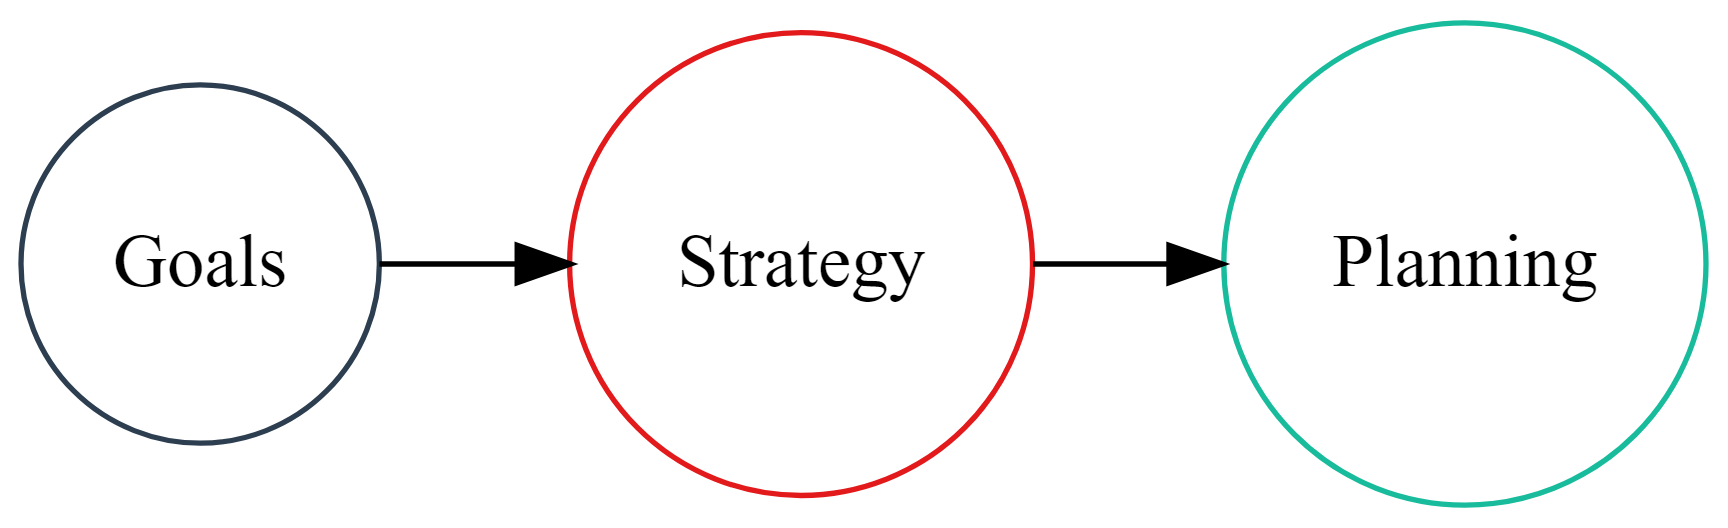
\includegraphics[width=4.5in,height=2.5in]{004_stra_plan_files/figure-beamer/dot-figure-1.png}

}

\caption{\label{fig-relation-ship-key-steps-planning-process}Relationship
between key steps in the planning process
(\citeproc{ref-lewicki_negociacion_2024}{Lewicki, Barry, and Saunders
2024, chap. 4}, p 105)}

\end{figure}%
\end{frame}

\section{Goals}\label{goals}

\begin{frame}{}
\phantomsection\label{section-5}
\begin{itemize}
\item
  The first step to execute a negotiation strategy is to determine one's
  goals.

  \begin{itemize}
  \tightlist
  \item
    \textbf{Substantive}: goals about tangible factors (price, terms of
    a contract, product specifications)
  \item
    \textbf{Intangible}: goals about intangible factors (personal values
    and emotions of the parties such as defeating the other party or
    reaching a conciliation at any cost)
  \item
    \textbf{Procedural}: goals about how the negotiation process occurs
    (define plans or just have a voice during the negotiation)
  \end{itemize}
\item
  The negotiator must identify what kind of goals to
  pursue\footnote<.->{Identifying goals in practical terms simply means
    making a list to prioritize them}. What definitely cannot be ignored
  is the substantive goals given that it refers to the tangible aspects.
\end{itemize}
\end{frame}

\begin{frame}{}
\phantomsection\label{section-6}
\begin{itemize}
\item
  When defining goals take into account these 4 aspects
  (\citeproc{ref-lewicki_negociacion_2024}{Lewicki, Barry, and Saunders
  2024, chap. 4}, p 105-106):

  \begin{itemize}
  \item
    Goals are specific objectives that are sought realistically.
  \item
    Own goals can potentially be linked to the goals of the other
    parties.\footnote<.->{It is easier to reach an agreement if you have
      common goals}
  \item
    If in identifying the goals these are not attainable then:

    \begin{itemize}
    \tightlist
    \item
      Modify them so that they are attainable
    \item
      Discard the negotiation as an option to reach an
      agreement\footnote<.->{Remember that negotiation as a form of
        \textbf{decision making} is not the only method that exists!}
    \end{itemize}
  \item
    The goals that are identified must be concrete, specific and
    measurable so that it is easier to:

    \begin{itemize}
    \tightlist
    \item
      Communicate to the other party what you want to achieve
    \item
      Understand what the other parties want
    \item
      Determine if the proposed proposals satisfy what you want to
      achieve
    \end{itemize}
  \end{itemize}
\end{itemize}
\end{frame}

\section{Strategies}\label{strategies}

\begin{frame}{}
\phantomsection\label{section-7}
\begin{figure}

\centering{

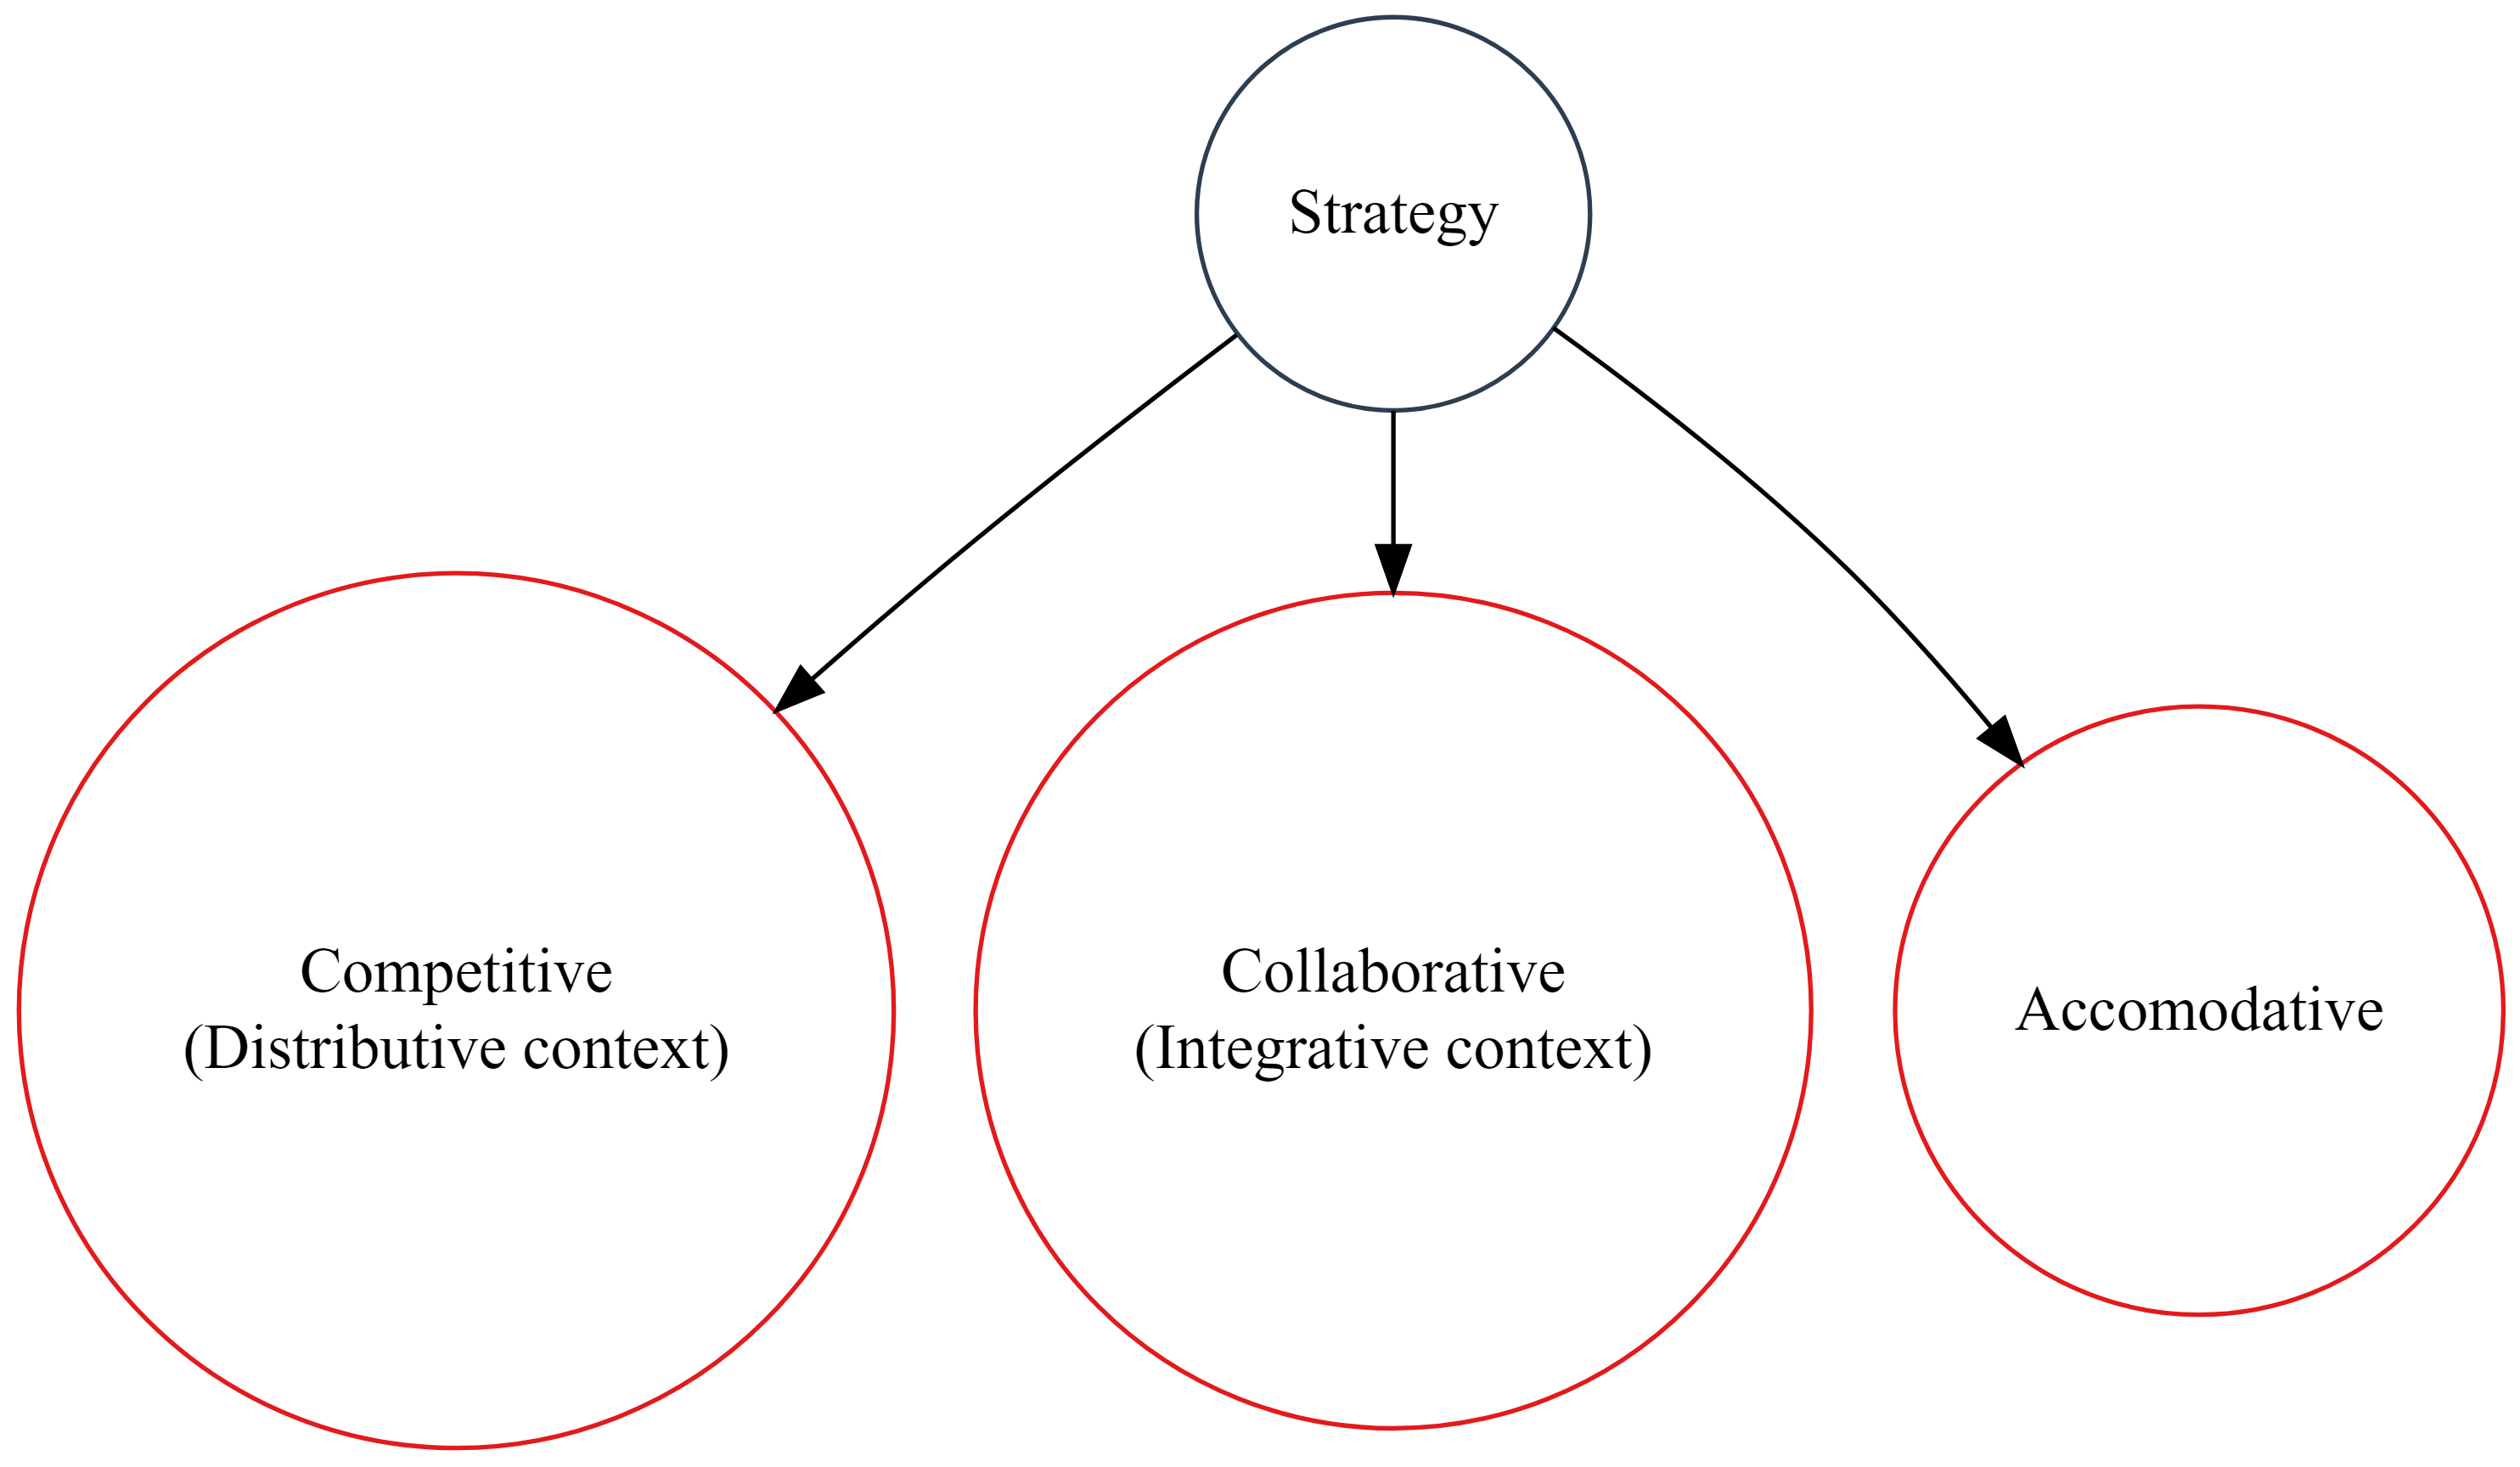
\includegraphics[width=5.5in,height=2.5in]{004_stra_plan_files/figure-beamer/dot-figure-4.png}

}

\caption{\label{fig-engagement-strategies}Different engagement
strategies in a negotiation context
(\citeproc{ref-lewicki_negociacion_2024}{Lewicki, Barry, and Saunders
2024, chap. 4}, p 110)}

\end{figure}%
\end{frame}

\section{Phases of negotiation}\label{phases-of-negotiation}

\begin{frame}{}
\phantomsection\label{section-8}
\begin{itemize}
\item
  Before exploring the specific planning processes for negotiation, it
  is important to understand the typical phases in a negotiation

  \begin{itemize}
  \item
    7 key steps to an ideal negotiation process
    (\citeproc{ref-greenhalgh_managing_2001}{Greenhalgh 2001}, p 164):

    \begin{itemize}
    \tightlist
    \item
      Preparation
    \item
      Relationship building
    \item
      Information gathering
    \item
      Information using
    \item
      Bidding
    \item
      Closing the deal
    \item
      Implementing the agreement
    \end{itemize}
  \end{itemize}
\end{itemize}
\end{frame}

\section{Planning process}\label{planning-process}

\begin{frame}{}
\phantomsection\label{section-9}
\begin{figure}

\centering{

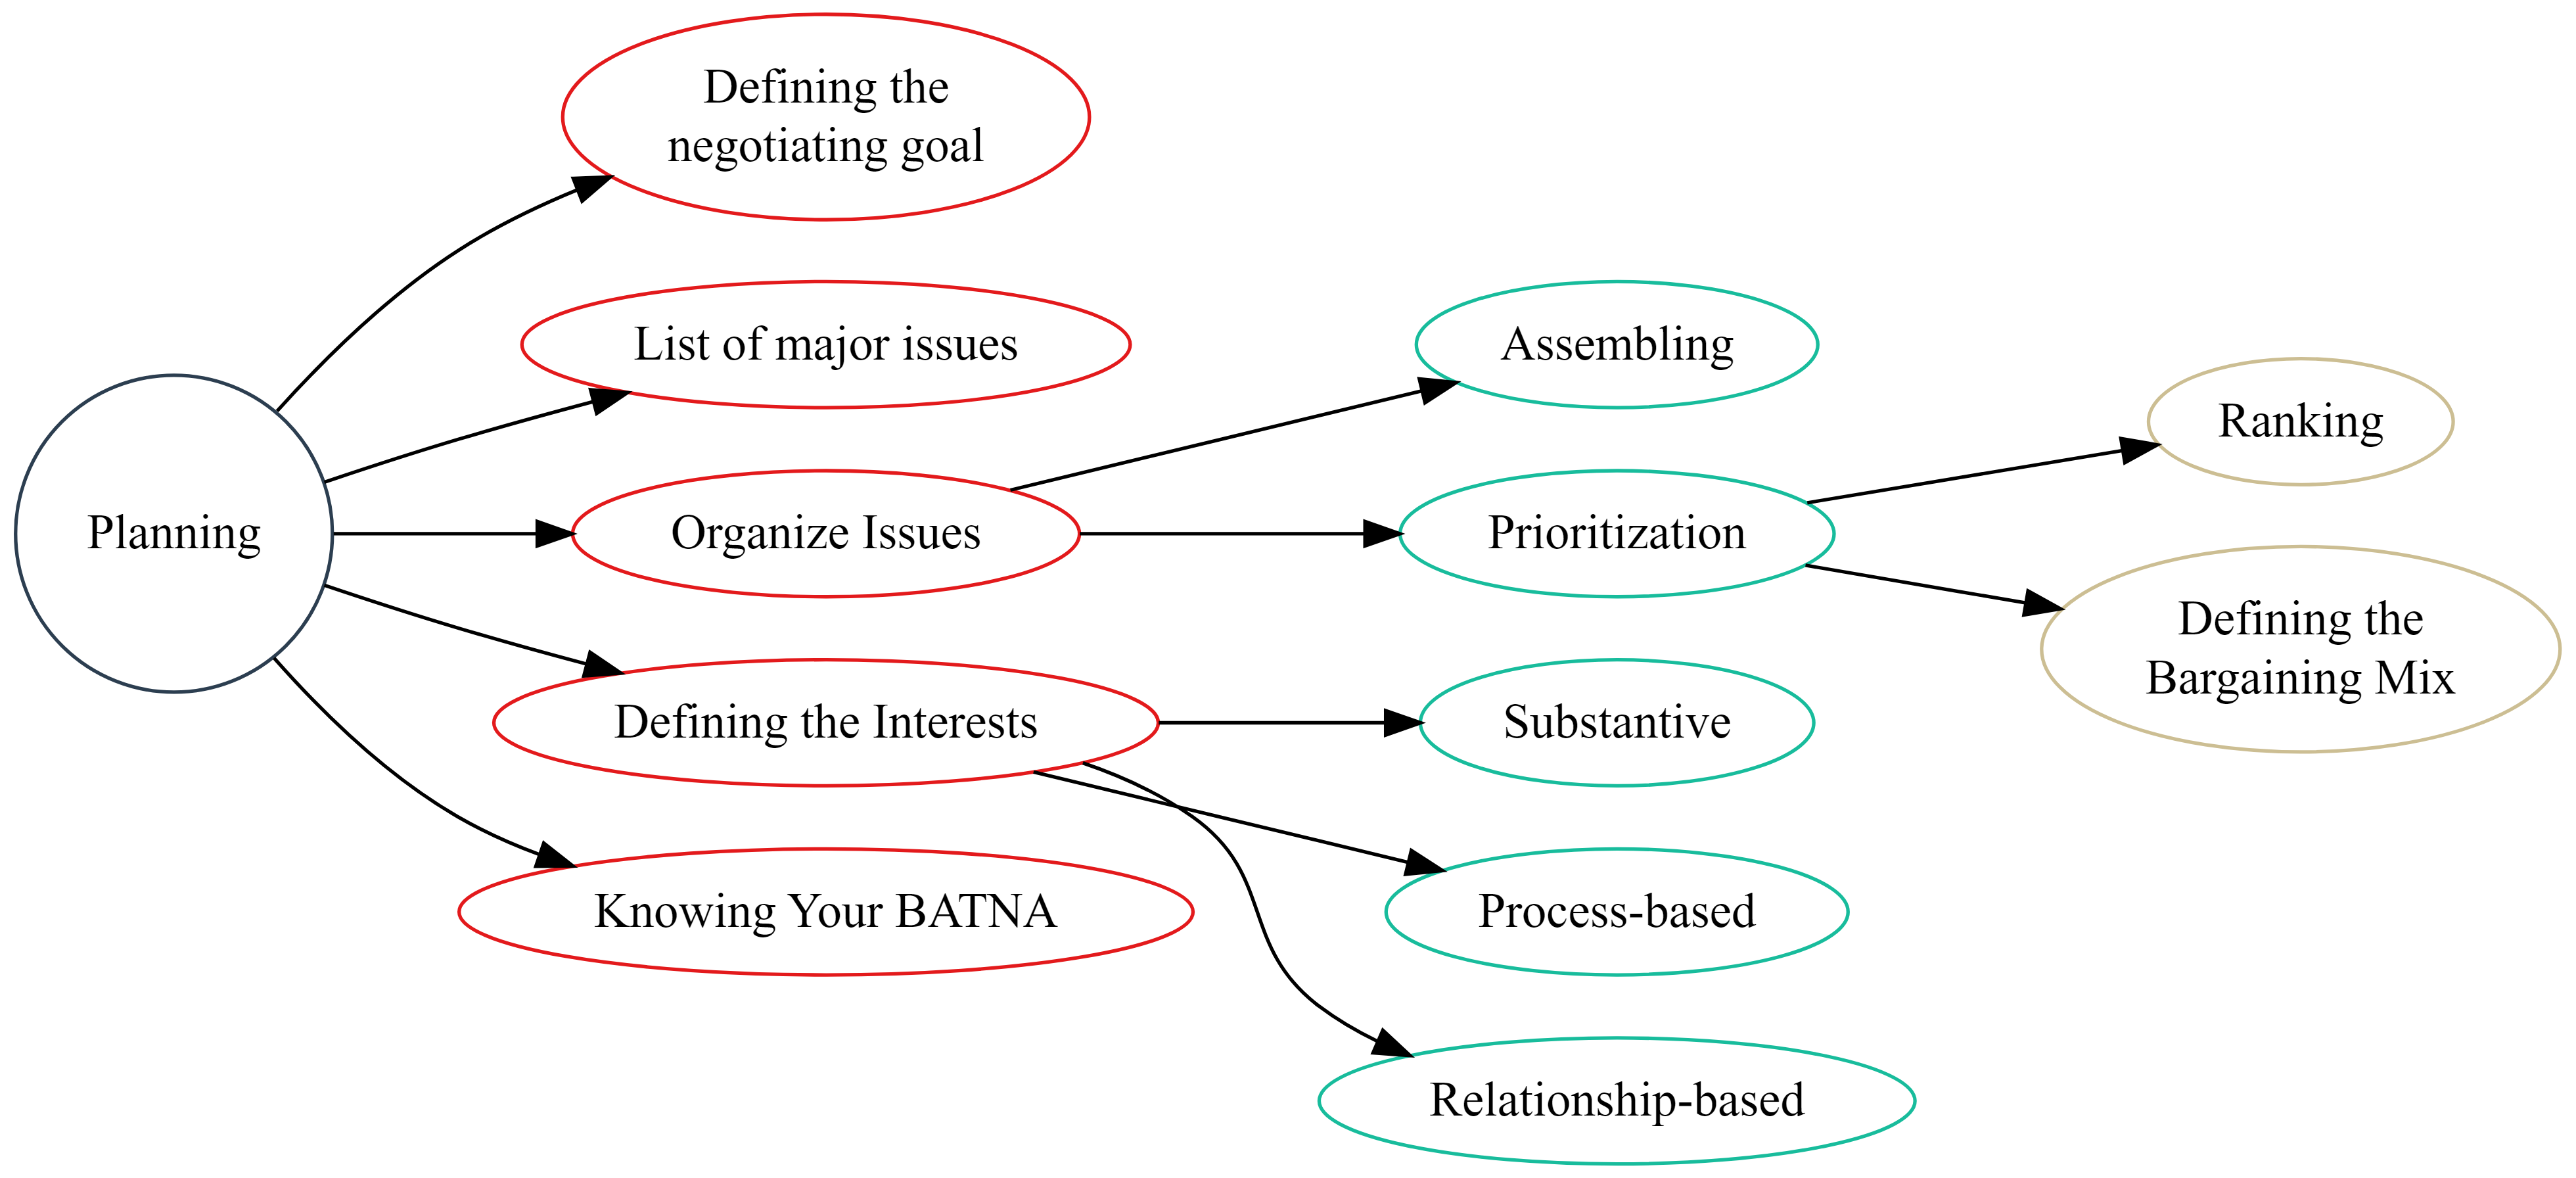
\includegraphics[width=4.5in,height=2.5in]{004_stra_plan_files/figure-beamer/dot-figure-3.png}

}

\caption{\label{fig-key-steps-planning-process-1}Key steps in the
planning process (\citeproc{ref-lewicki_negociacion_2024}{Lewicki,
Barry, and Saunders 2024, chap. 4}, p 114-128)}

\end{figure}%
\end{frame}

\begin{frame}{}
\phantomsection\label{section-10}
\begin{figure}

\centering{

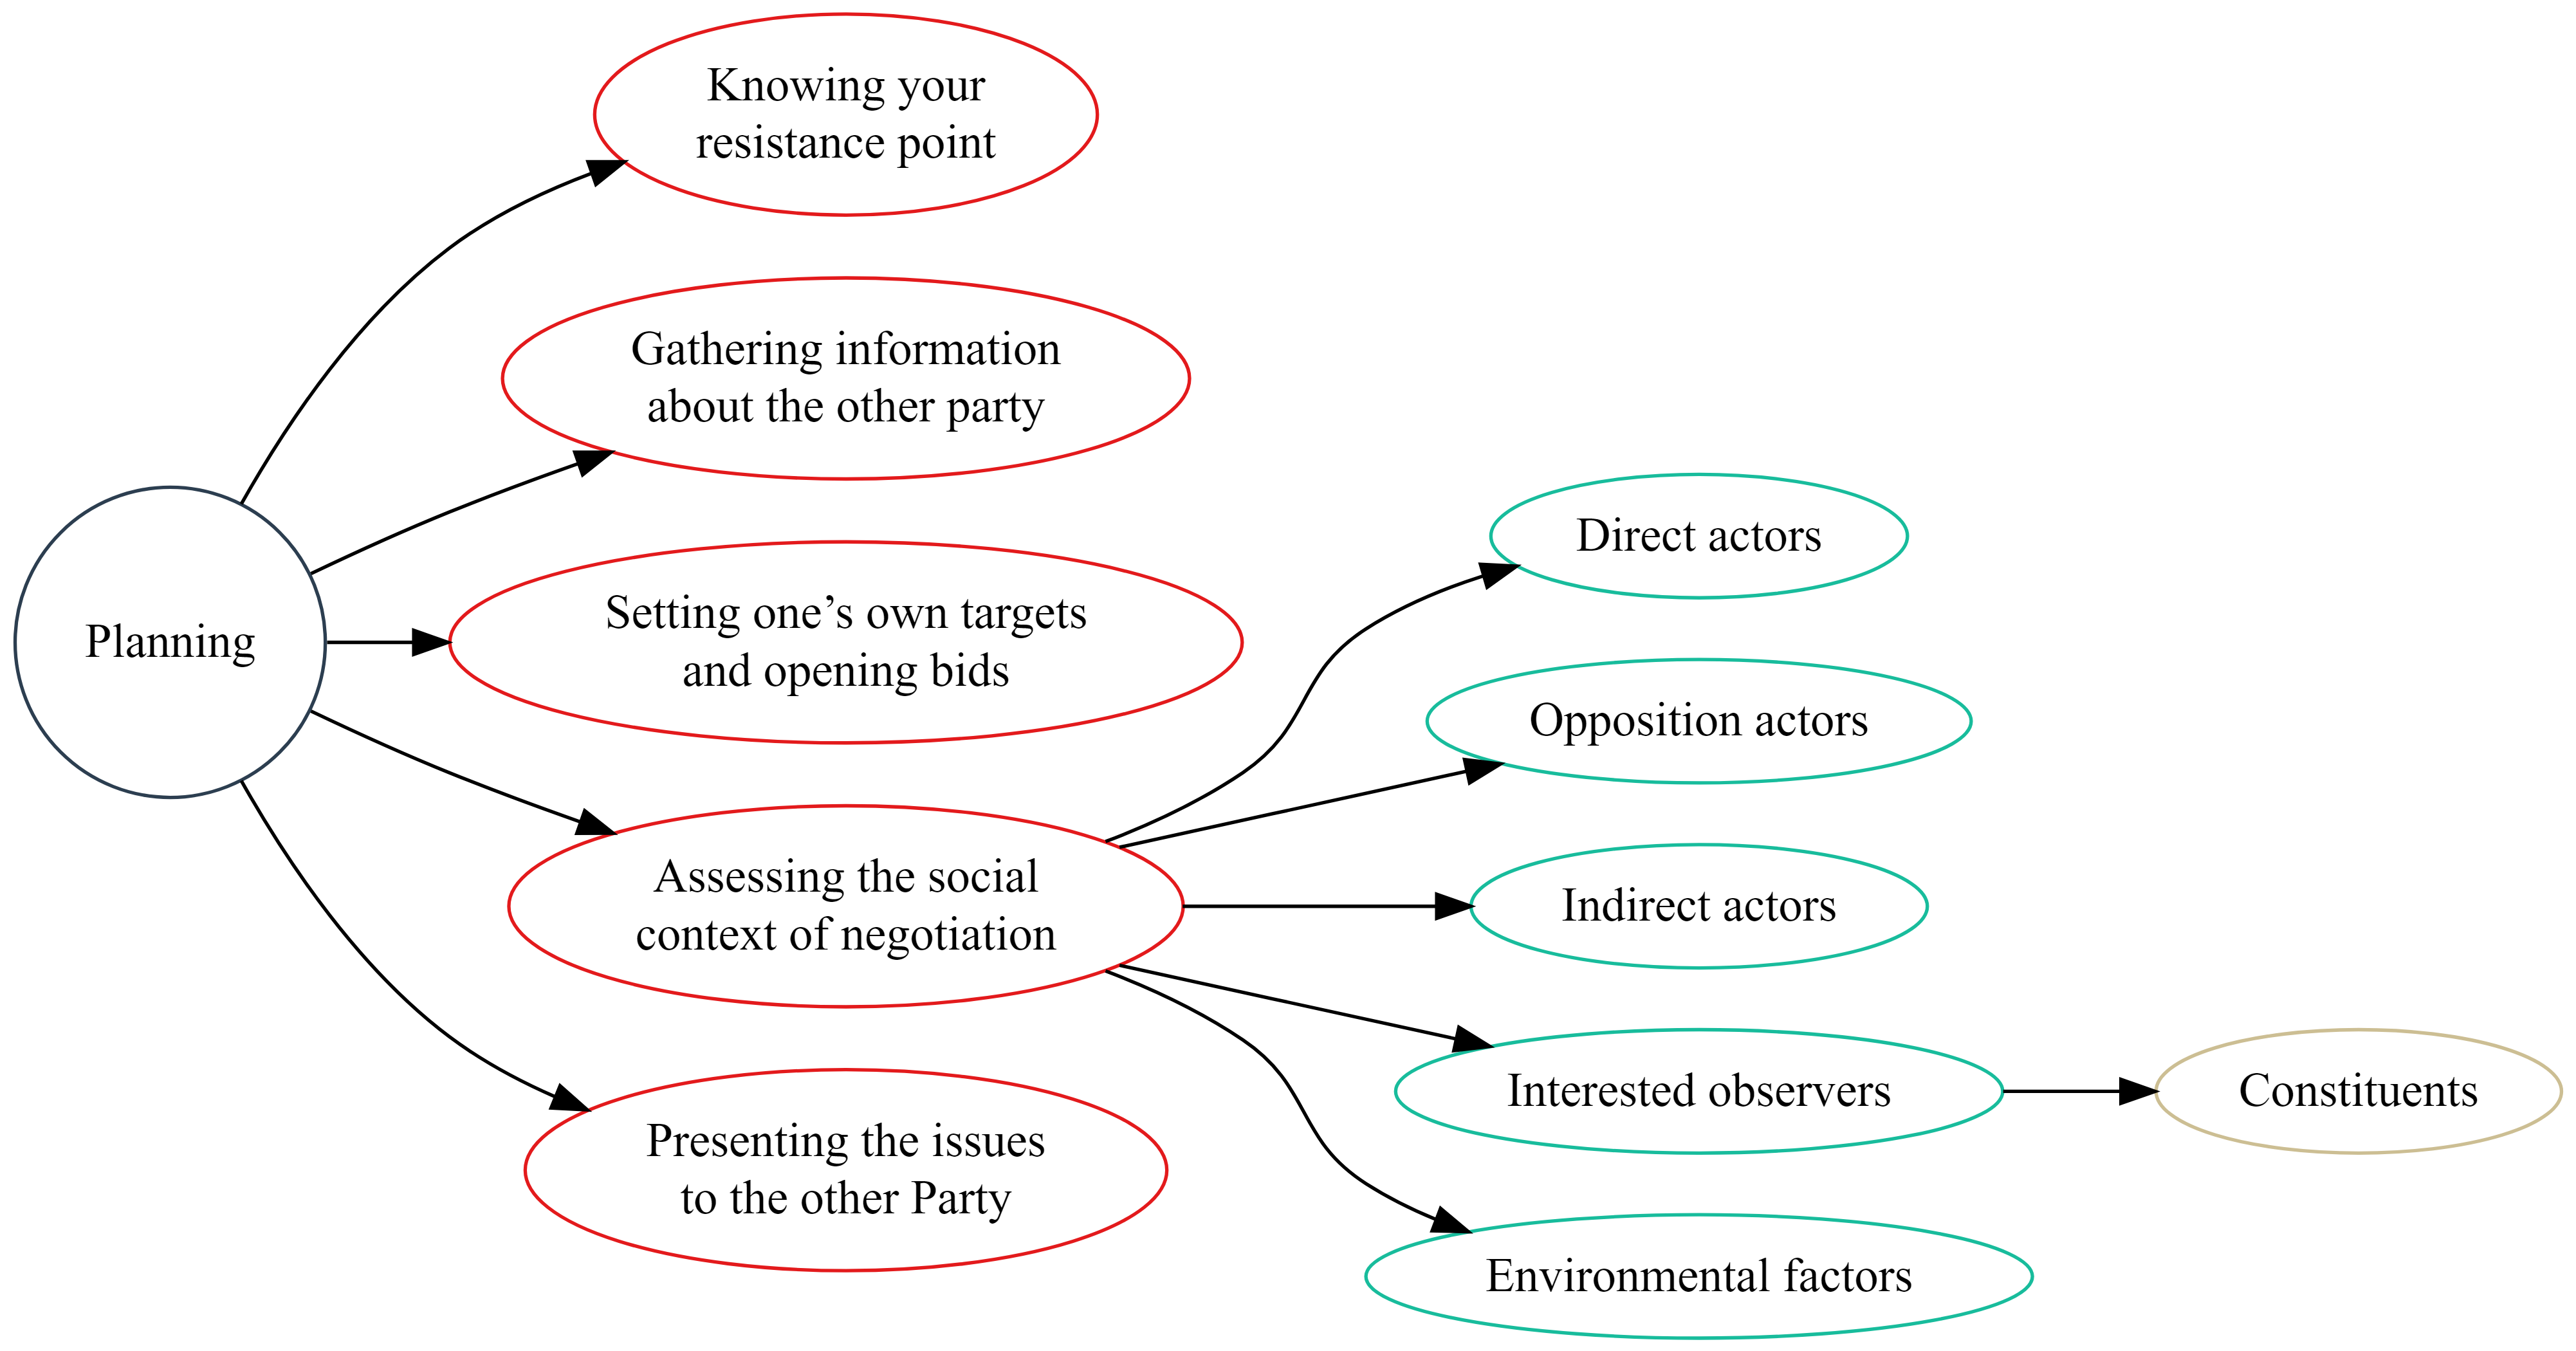
\includegraphics[width=5.5in,height=2.5in]{004_stra_plan_files/figure-beamer/dot-figure-2.png}

}

\caption{\label{fig-key-steps-planning-process-2}Key steps in the
planning process (\citeproc{ref-lewicki_negociacion_2024}{Lewicki,
Barry, and Saunders 2024, chap. 4}, p 114-128)}

\end{figure}%
\end{frame}

\section{Acknowledgments}\label{acknowledgments}

\begin{frame}{}
\phantomsection\label{section-11}
\begin{itemize}
\item
  To my family that supports me
\item
  To the taxpayers of Colombia and the
  \href{https://www.umng.edu.co/estudiante}{\textbf{UMNG students}} who
  pay my salary
\item
  To the \href{https://www.business-science.io/}{\textbf{Business
  Science}} and \href{https://www.rfordatasci.com/}{\textbf{R4DS Online
  Learning}} communities where I learn
  \href{https://www.r-project.org/about.html}{\textbf{R}} and
  \href{https://www.python.org/about/}{\textbf{\(\pi\)-thon}}
\item
  To the \href{https://www.r-project.org/contributors.html}{\textbf{R
  Core Team}}, the creators of
  \href{https://rstudio.com/products/rstudio/}{\textbf{RStudio IDE}},
  \href{https://quarto.org/}{\textbf{Quarto}} and the authors and
  maintainers of the packages
  \href{https://CRAN.R-project.org/package=tufte}{\textbf{tufte}} and
  \href{https://CRAN.R-project.org/package=tinytex}{\textbf{tinytex}}
  for allowing me to access these tools without paying for a license
\item
  To the \href{https://www.kernel.org/category/about.html}{\textbf{Linux
  kernel community}} for allowing me the possibility to use some
  \href{https://static.lwn.net/Distributions/}{\textbf{Linux
  distributions}} as my main
  \href{https://en.wikipedia.org/wiki/Operating_system}{\textbf{OS}}
  without paying for a license
\end{itemize}
\end{frame}

\section*{References}\label{references}
\addcontentsline{toc}{section}{References}

\begin{frame}[allowframebreaks]{References}
\phantomsection\label{refs}
\begin{CSLReferences}{1}{0}
\bibitem[\citeproctext]{ref-greenhalgh_managing_2001}
Greenhalgh, Leonard. 2001. \emph{Managing Strategic Relationships: The
Key to Business Success}. New York: Free Press.

\bibitem[\citeproctext]{ref-lewicki_negociacion_2024}
Lewicki, Roy J., Bruce Barry, and David M. Saunders. 2024.
\emph{Negociación}. 9th ed. McGraw-Hill Education.
\url{https://www-ebooks7-24-com.ezproxy.umng.edu.co/?il=40562}.

\bibitem[\citeproctext]{ref-magic_markers_como_2018}
Magic Markers. 2018. {``¿{Cómo} Negociar Bien?''}
\url{https://youtu.be/CnF26cfIfQM}.

\bibitem[\citeproctext]{ref-rackham_effective_1978-1}
Rackham, Neil, and John Carlisle. 1978a. {``The {Effective} {Negotiator}
--- {Part} {I}: {The} {Behaviour} of {Successful} {Negotiators}.''}
\emph{Journal of European Industrial Training} 2 (6): 6--11.
\url{https://doi.org/10.1108/eb002297}.

\bibitem[\citeproctext]{ref-rackham_effective_1978}
---------. 1978b. {``The {Effective} {Negotiator} --- {Part} 2:
{Planning} for {Negotiations}.''} \emph{Journal of European Industrial
Training} 2 (7): 2--5. \url{https://doi.org/10.1108/eb002302}.

\end{CSLReferences}
\end{frame}




\end{document}
